\documentclass[ex, minted]{exercise_4.1}

\deadline{10.07.2024}

\begin{document}

\section{Formfaktor}
{\it Bei der elastischen Elektron-Kern-Streuung führt die ausgedehnte Ladungsverteilung des Kernes zu einer Modifikation des Mott/Rutherford-Streuquerschnittes, die durch einen Formfaktor ausgedrückt werden kann. Berechnen Sie den Formfaktor für }

\subsection{ein punktförmiges Target.}

\dottedlinete

\begin{align*}
    F(q) 
    &= \int e^{i \v q\cdot \v x / \hbar } \rho(\v x) \dv x
    = \int e^{i \v q\cdot \v x / \hbar } \delta(\v x ) \dv x= 1
\end{align*}

\subsection{einen kugelförmigen Kern mit Radius \(R\) und konstanter Ladungsdichte.}

\dottedlinett

Allgemein gilt für eine kugelsymmetrische Ladungsverteilung:
\begin{align*}
    F(\v q) 
    &= \int \rho(r) e^{i \v q\cdot \v x / \hbar }\d{^3r}\\
    &= \int \rho(r) e^{i q r \cos\theta / \hbar }\d{^3r}\\
    &= 2\pi \int_0^\inf \dr r^2 \rho(r) \int_{-1}^1\d{\cos\theta}  e^{i q r\cos\theta / \hbar}\\
    &= 2\pi \int_0^\inf \dr r^2\rho(r)  \frac{\hbar}{i q r}e^{i q r\cos\theta / \hbar}\eval_{-1}^1\\
    &= \frac{4\pi\hbar}{q}\int_0^\inf \dr r\rho(r) \frac{1}{2i}e^{i q r\cos\theta / \hbar }\eval_{-1}^1\\
    &= \frac{4\pi\hbar}{q}\int_0^\inf \dr r \rho(r) \sin\hug{q r/ \hbar }\\
\end{align*}
Und damit für die homogen geladene Kugel:
\begin{align*}
    \rho(r) &= \frac{\Theta(R-r)}{\frac43 \pi R^3}\\
    F(\v q) &= \frac{4\pi\hbar}{q} \frac{1}{\frac43 \pi R^3}\intr r \sin\hug{q r/ \hbar }\\
    &= \frac{3}{R^3} \frac{\hbar}{q}\intr r \sin\hug{q r/ \hbar }\\
    &= \frac{3}{R^3} \frac{\hbar}{q}\intr r \sin\hug{q r/ \hbar }\\
    &= \frac{3}{R^3} \frac{\hbar}{q}\hug{-\frac\hbar q r \cos\hug{q r/ \hbar } + \frac\hbar q \int \dr \cos(qr/\hbar)}\eval_0^R\\
    &= \frac{3}{R^3} \frac{\hbar}{q}\hug{-\frac\hbar q R \cos\hug{q R/ \hbar } + \frac{\hbar^2}{q^2} \sin(qr/\hbar)\eval_0^R}\\
    &= \frac{3}{R^3} \frac{\hbar}{q}\hug{-\frac\hbar q R \cos\hug{q R/ \hbar } + \frac{\hbar^2}{q^2} \sin(qR/\hbar)}\\
    &= \frac{3}{\epsilon^3}\hug{\sin\epsilon - \epsilon \cos\epsilon}\with \epsilon = \frac{qR}{\hbar}
\end{align*}

\section{Streuexperiment an einer harten Kugel}
{\it In der Vorlesung haben Sie die semi-klassische Berechnung der Rutherford-Streuung kennen gelernt. Hier werden Sie diese Berechnung für die Streuung einer harten Kugel anwenden. Statt einem abstoßendem Coulomb Potential können Sie ein abstoßendes Potential der Form 
\begin{align*}
    V(r) = \begin{cases}
        \inf, &r\le a\\
        0, &r>a
    \end{cases}
\end{align*}
annehmen. Die einfallenden Teilchen werden im folgenden als Punkte ohne räumliche Ausdehnung angenommen.
}

\subsection{Nutzen Sie die Abbildung 1 und bestimmen Sie das Verhältnis der Streuwinkel \(\theta\) mit dem Stoßparameter \(b\) und geben Sie die Gleichung \(b(\theta)\) an.}

\dottedlinett

Aus der Skizze
\begin{figure}[H]
    \centering
    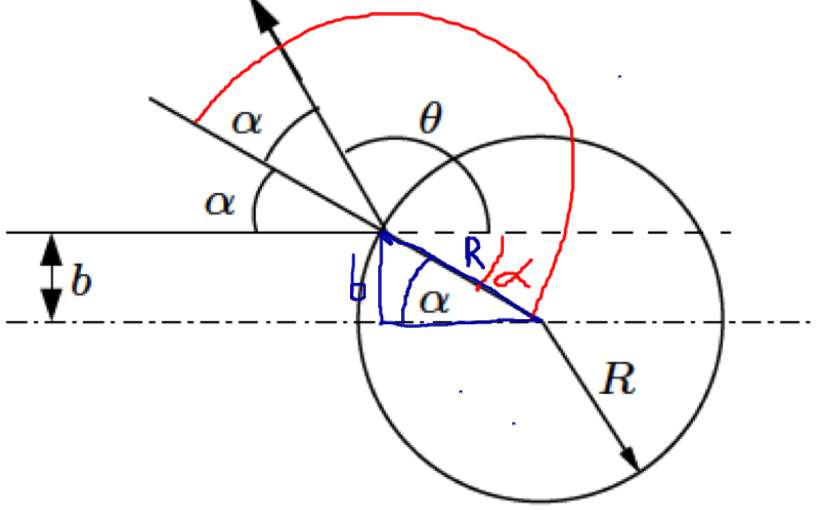
\includegraphics[width=.5\textwidth]{skizze.png}
    \caption{Skizze mit Einzeichnungen}
\end{figure}
lassen sich die beiden Zusammenhänge 
\begin{align*}
    \theta &= \pi - 2\alpha\tand \sin \alpha = \frac b R  
\end{align*}
ablesen, folglich ist 
\begin{align*}
    b = R\sin\hug{\frac{\pi-\theta}{2}} = R\cos\hug{\frac \theta 2}
\end{align*}

\subsection{Gehen Sie analog zur Herleitung der Rutherfordsche Streuformel vor und leiten Sie den differenziellen Wirkungsquerschnitt \(\dd \sigma \Omega\) her. }

\dottedlinett

\begin{align*}
    \pp \sigma \Omega 
    &= \abs{\pp \sigma b}\cdot \abs{\pp b \theta }\cdot \abs{\pp \theta \Omega}\\
    \d\Omega &= \sin\theta \dtheta \dphi=2\pi \sin\theta \dtheta\implies \dd \theta\Omega = \frac{1}{2\pi \sin \theta }= \frac{1}{4\pi \sin\frac\theta2 \cos\frac\theta 2}
    \\
    &= 2\pi b(\theta)\cdot\frac R2 \sin\hug{\frac \theta 2}\cdot \frac{1}{4\pi \sin\frac\theta2 \cos\frac\theta 2}\\
    &= 2\pi R\cos\hug{\frac \theta 2}\cdot\frac R2 \sin\hug{\frac \theta 2}\cdot \frac{1}{4\pi \sin\frac\theta2 \cos\frac\theta 2}\\
    &= \frac {R^2} 4
\end{align*}

\subsection{Berechnen Sie aus dem Ergebnis des vorherigen Aufgabenteils den totalen Wirkungsquerschnitt und vergleichen Sie das Ergebnis mit der Geometrie der Kugel.}

\dottedlinete

\begin{align*}
    \sigma 
    &= \int_{4\pi} \dd \sigma \Omega \d\Omega \\  
    &= \dd \sigma \Omega\int_{4\pi} \d\Omega \\  
    &= \pi R^2
\end{align*}
Der totale Wirkungsquerschnitt entspricht somit der Querschnittsfläche der Kugel.

\subsection{Nehmen Sie jetzt an, dass das Material, an dem gestreut wird, zu einem Anteil \(x\) aus Kugeln mit dem Radius \(R_a\) und einem Anteil \(1-x\) aus Kugeln mit dem Radius \(R_b\) besteht. Was ist der differenzielle Wirkungsquerschnitt für dieses Material? Was wäre der differenzielle Wirkungsquerschnitt für Radien die nach einer Funktion \(p(r)\) verteilt sind?}

\dottedlinett

Sofern das Material keine Dicke hat, kann einfach der Erwartungswert  des differenziellen Wirkungsquerschnitte ermittelt werden:
\begin{align*}
    \pp \sigma \Omega (R) &= \frac {R^2} 4\\
    \pp \sigma \Omega &= \int p(R) \pp \sigma \Omega (R)\d R\\
    \\
    p(R) &= x \delta(R_a-R) + (1-x)\delta(R_b-R)\\
    \implies \pp \sigma \Omega &= x\frac{R_a}{2} + (1-x)\frac{R_b}{2}
\end{align*}

\newpage
\section{Rutherford Streuung}
\subsection{Lesen Sie die Daten aus der Datei Rutherford.csv aus und plotten Sie die Winkelverteilung der Streuung mit den geeigneten Daten.\\
Hinweis: Beachten die unterschiedliche Messdauern der Einzelmessungen.}

\dottedlinett

\inputpy[firstline=2,lastline=12]{}{12.py}
\begin{figure}[H]
    \centering
    \includesvg[width=.5\textwidth]{1.svg}
    \caption{Resultierender Plot}
\end{figure}

\subsection{Fitten Sie das Streumodell an die Daten 
\begin{align*}
    \dd \sigma \Omega = a \sin (\theta/2)^b
\end{align*} Stellen Sie das Ergebnis ebendfalls grafisch dar.\\
Hinweis: Wählen Sie auch eine geeignete Darstellung der Achsen, so dass ihr Ergebnis möglich gut repräsentiert wird.
}

\dottedlinett

\inputpy[firstline=15,lastline=28]{}{12.py}

\begin{figure}[H]
    \centering
    \includesvg[width=.5\textwidth]{2.svg}
    \caption{Resultierender Plot}
\end{figure}

\section{Isospin des Deuterons}
{\it Der Isospin is ein kernphysikalisches Konzept, das die Symmetrie der starken Wechselwirkung gegen Vertauschung von Proton und Neutron beschreibt und dabei auf die Analogie der Symmetrie der elektromagnetischen Wechselwirkung gegen Spin up und Spin down zurückgreift um auf algrebraisch gleiche Rechenregeln zu schließen.}

\subsection{Zeigen Sie zunächst qualitativ, dass der Isospin des Deuterons Null ist. Begründen Sie dies aus zwei verschiedenen Gesichtspunkten:}

\subsubsection{Aus der experimentellen Beobachtung.}

\dottedlinett

Chemische Eigenschaften von Wasserstoff \(\to\) Ein Proton im Kern; Jedoch ungefähr doppelte Masse \(\to\) weiter ein Neutron im Kern. Insgesamt also Isospin gleich null.

\subsubsection{Durch die Anwendung des Pauliprinzips, das besagt, dass die gesamte Wellenfunktion, die ein Produkt aus Orts-, Spin- und Isospin-anteil sein soll, antisymmetrisch bezüglich des Austauschs zweier
Nukleonen sein muss.}

\dottedlinett

Der Raumanteil der Wellenfunktion ist symmetrisch (vorwiegend \(L=0\)), beim Spin liegt ein Triplett vor (symmetrisch; energetisch günstiger), weshalb die gesamte Wellenfunktion nur antisymmetrisch unter dem Permutationsoperator ist, wenn der Isospin verschwindet (antisymmetrisch).

\subsection{In Reaktionen der starken Wechselwirkung ist der Gesamt-Isospin erhalten, in Analogie zur Erhaltung
des Gesamtspins. Die Kern-Reaktion
\begin{align*}
    dd \to \alpha \pi^0
\end{align*}
wird in der Natur nicht beobachtet. Wenn der Isospin des Deuterons und des \(\alpha\)-Teilchens Null ist, was besagt das Fehlen dieser Reaktion für den Isospin des Pions?}

\dottedlinett

Wenn die Kern-Reaktion \(dd \to \alpha \pi^0\) in der Natur nicht vorkommt, ist das ein Hinweis darauf, dass der Isospin des Pion ungleich null ist, weil der Übergang dann nach der Isospinerhaltung nicht über die starke (oder Coloumb-/) Wechselwirkung möglich wäre. 


\end{document}